%+TITLE: Repaso de relatividad especial
%+DESCRIPTION: Hacemos un repaso de la relatividad especial para estudiar luego el grupo de Lorentz
\documentclass[11pt,a4paper]{article}

\usepackage[utf8]{inputenc}
\usepackage[T1]{fontenc}
\usepackage[spanish,es-nodecimaldot]{babel}
\usepackage{lmodern}
\usepackage{amsmath,amssymb,mathtools}
\usepackage{graphicx}
\usepackage{xcolor}
\usepackage{geometry}
\usepackage{enumitem}
\usepackage{microtype}

\geometry{margin=2.3cm}
\setlength{\parindent}{0pt}
\setlength{\parskip}{0.65em}
\setlist[itemize]{leftmargin=1.6em,itemsep=0.25em,topsep=0.25em}

\definecolor{title-red}{RGB}{165,25,20}
\definecolor{concept-green}{RGB}{20,125,45}
\newcommand{\concept}[1]{\textcolor{concept-green}{#1}}

\newcommand{\ket}[1]{\left|#1\right\rangle}
\newcommand{\bra}[1]{\left\langle#1\right|}
\newcommand{\braket}[2]{\left\langle #1\middle|#2\right\rangle}
\newcommand{\hc}{\mathrm{h.c.}}
\newcommand{\Tr}{\operatorname{Tr}}
\newcommand{\Diffs}{\mathrm{Diffs}}

\begin{document}

En las ecuaciones de Maxwell aparece una velocidad absoluta $c$. Pero nuestra intuición nos dice que, si un objeto tiene una velocidad $\vec v$ en un marco de referencia, entonces en otro marco de referencia inercial que se mueve con velocidad $\vec w$ respecto al primero la velocidad será
\[
  \vec v'=\vec v+\vec w.
\]

Eso quiere decir que no hay velocidades absolutas, tal que las ecuaciones de Maxwell parecen escritas en un marco de referencia especial (el éter). Si eso es así, la velocidad de la luz debería ser diferente para distintos marcos de referencia. Pero esto nunca se observó en un experimento.

Einstein le dio la vuelta al argumento. Lo que está mal es la suma de velocidades. Propuso una velocidad máxima igual en todos los marcos de referencia: la velocidad de la luz.

Esto es muy contrario a nuestra intuición. Consideremos un rayo de luz que rebota entre dos espejos para un observador $O$ en reposo respecto a los espejos.

\begin{center}
  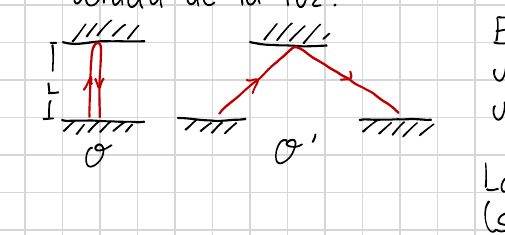
\includegraphics[width=0.47\linewidth]{figures/reloj_de_luz.png}
\end{center}

La luz tarda un tiempo
\[
  \Delta t=\frac{2L}{c}
\]
en ir y volver (según $O$).

Pero para $O'$ la distancia que tiene que recorrer la luz es mayor:
\[
  2\sqrt{L^2+\frac{w^2\Delta t'^2}{4}}.
\]
Por tanto,
\begin{align*}
  \Delta t'
  &=\frac{2}{c}\sqrt{L^2+\frac{w^2\Delta t'^2}{4}}, \\
  \frac{\Delta t'^2}{4}(c^2-w^2)&=L^2,
\end{align*}
y entonces
\[
  \Delta t'
  =\frac{1}{\sqrt{1-w^2/c^2}}\left(\frac{2L}{c}\right)
  =\frac{1}{\sqrt{1-w^2/c^2}}\,\Delta t.
\]

Haciendo experimentos mentales, como este, podemos deducir la relación entre marcos de referencia. Aquí lo haremos de otra manera. Con este y otros ejemplos se ve que ni el tiempo ni la magnitud del vector posición permanecen invariantes bajo cambio de marco. Lo que permanece invariante es
\[
  \Delta s^2=-c^2\Delta t^2+|\Delta\vec X|^2
  \qquad\longrightarrow\qquad
  \concept{\text{intervalo entre eventos}}.
\]

Para un rayo de luz (o cualquier partícula sin masa), $\Delta s^2=0$.

Buscamos las transformaciones que dejan invariante el intervalo. Ya conocemos algunas, que no tocan el tiempo y sólo cambian $\Delta\vec X$:

\begin{itemize}
  \item Traslaciones espaciales:
  \[
    t\mapsto t'=t,
    \qquad
    \vec X\mapsto\vec X'=\vec X+\vec a.
  \]
  Claramente,
  \[
    \Delta t=\Delta t',
    \qquad
    \Delta\vec X
    =\vec X_2-\vec X_1
    =\vec X_2'-\vec a-\vec X_1'+\vec a
    =\Delta\vec X',
  \]
  de modo que $\Delta s^2=\Delta s'^2$. Son tres: traslaciones en $x,y,z$.

  \item Rotaciones:
  \[
    t\mapsto t'=t,
    \qquad
    \vec X\mapsto\vec X'=R_{\hat n}(\theta)\vec X.
  \]
  Ya vimos que son tres y que $|\Delta\vec X|^2=|\Delta\vec X'|^2$.
  Claramente, $\Delta t=\Delta t'$, luego $\Delta s^2=\Delta s'^2$.
\end{itemize}

Otra muy sencilla es no transformar $\vec X$ y sumarle una constante a $t$.

\begin{itemize}
  \item Traslaciones temporales:
  \[
    t\mapsto t'=t+a^0,
    \qquad
    \vec X\mapsto\vec X'=\vec X.
  \]
  \[
    \Delta t'=t_2'-t_1'=t_2+a^0-t_1-a^0=\Delta t,
    \qquad
    \Delta\vec X'=\Delta\vec X,
  \]
  por lo que $\Delta s'^2=\Delta s^2$.
\end{itemize}

Hay otras transformaciones. Notemos que
\[
  \Delta s^2=-c^2\Delta t^2+\Delta x^2+\Delta y^2+\Delta z^2
\]
es la ecuación de un hiperboloide. Los senos y cosenos hiperbólicos satisfacen ese tipo de ecuación,
\[
  1=\cosh^2\alpha-\sinh^2\alpha,
\]
por eso se llaman así. Entonces, por ejemplo, nos inspiramos en las rotaciones para escribir
\[
  t\mapsto t'=\cosh\alpha\,t+\sinh\alpha\,\frac{x}{c},
  \qquad
  x\mapsto x'=\sinh\alpha\,ct+\cosh\alpha\,x,
  \qquad
  y'=y,
  \qquad
  z'=z.
\]

En efecto,
\begin{align*}
  -c^2\Delta t'^2+\Delta x'^2
  &=-\bigl(\cosh\alpha\,c\Delta t+\sinh\alpha\,\Delta x\bigr)^2
    +\bigl(\sinh\alpha\,c\Delta t+\cosh\alpha\,\Delta x\bigr)^2 \\
  &=-\Delta t^2c^2(\cosh^2\alpha-\sinh^2\alpha)
    +\Delta x^2(\cosh^2\alpha-\sinh^2\alpha) \\
  &=-c^2\Delta t^2+\Delta x^2.
\end{align*}

¿Cuál es el significado físico de esta transformación? Consideremos el origen del sistema $O'$, es decir, $\Delta x'=0$, tal que
\[
  \sinh\alpha\,c\Delta t=-\cosh\alpha\,\Delta x
  \quad\Longrightarrow\quad
  w=\frac{\Delta x}{\Delta t}=-c\tanh\alpha.
\]

Entonces $\alpha$ está relacionada con la velocidad del observador $O'$ respecto al observador $O$. Usando $\cosh^2\alpha-\sinh^2\alpha=1$,
\[
  \cosh^2\alpha
  =\frac{1}{1-\tanh^2\alpha}
  =\frac{1}{1-w^2/c^2},
  \qquad
  \cosh\alpha=\frac{1}{\sqrt{1-w^2/c^2}}=\gamma,
\]
\[
  \sinh\alpha=\cosh\alpha\tanh\alpha
  =-\gamma\frac{w}{c}=-\gamma\beta.
\]

Por tanto,
\[
  \Delta t'=\gamma\left(\Delta t-\beta\frac{\Delta x}{c}\right),
  \qquad
  \Delta x'=\gamma(\Delta x-\beta c\Delta t),
  \qquad
  \Delta y'=\Delta y,
  \qquad
  \Delta z'=\Delta z.
\]

\begin{itemize}
  \item ``Boosts'': son tres independientes (respecto a $x$, $y$ o $z$).
\end{itemize}

El ``boost'' es un cambio de marco de referencia hacia otro que se mueve a velocidad constante respecto al primero.

Notemos que la velocidad de la luz es la misma para todos los observadores. Por eso trabajamos con unidades tales que $c=1$ (unidades naturales).

Notemos también que los boosts mezclan el espacio y el tiempo. Por ejemplo, si para el observador $O$ dos eventos ocurren al mismo tiempo, $\Delta t=0$, para $O'$,
\[
  \Delta t'=-\beta\gamma\Delta x,
\]
de modo que los eventos no son simultáneos.

Decir que dos cosas ``ocurren al mismo tiempo'' no tiene sentido: depende del observador.

Como el espacio y el tiempo se mezclan, los tratamos al mismo nivel, tal que nuestro espacio-tiempo tiene coordenadas $X^\mu$, con $X^0=t$. Además, escribimos
\[
  \Delta s^2=\eta_{\mu\nu}\Delta X^\mu\Delta X^\nu,
  \qquad
  \eta^{\mu\nu}=
  \begin{pmatrix}
    -1&0&0&0\\
    0&1&0&0\\
    0&0&1&0\\
    0&0&0&1
  \end{pmatrix}
  \qquad\longrightarrow\qquad
  \concept{\text{métrica de Minkowski}}.
\]

Las rotaciones y boosts, que no involucran traslaciones, se llaman \concept{transformaciones de Lorentz}. Escribimos
\[
  X'^\mu=\Lambda^\mu{}_{\nu}X^\nu,
\]
y la invariancia del intervalo exige
\begin{align*}
  \eta_{\mu\nu}\Delta X'^\mu\Delta X'^\nu
  &=\eta_{\mu\nu}\Lambda^\mu{}_{\alpha}\Lambda^\nu{}_{\beta}
    \Delta X^\alpha\Delta X^\beta \\
  &=\eta_{\alpha\beta}\Lambda^\alpha{}_{\mu}\Lambda^\beta{}_{\nu}
    \Delta X^\mu\Delta X^\nu.
\end{align*}

Pero esto tiene que ser igual a $\eta_{\mu\nu}\Delta X^\mu\Delta X^\nu$ para
cualquier $\Delta X$, tal que
\[
  \eta_{\alpha\beta}\Lambda^\alpha{}_{\mu}\Lambda^\beta{}_{\nu}
  =\eta_{\mu\nu}.
\]

Esta es la condición que define el \concept{grupo de Lorentz} $O(1,3)$. Está dado por todas las matrices $4\times4$ que satisfacen
\[
  \Lambda^T\eta\Lambda=\eta.
\]

Tomando el determinante a ambos lados,
\[
  (\det\Lambda)^2=1,
  \qquad\text{tal que}\qquad
  \det\Lambda=\pm1.
\]

Como queremos estudiar las transformaciones infinitesimalmente cercanas a la identidad, consideramos sólo $\det\Lambda=1$, formando el grupo $SO(1,3)$. Esto excluye transformaciones como inversión temporal y paridad:
\[
  T=
  \begin{pmatrix}
    -1&0&0&0\\
    0&1&0&0\\
    0&0&1&0\\
    0&0&0&1
  \end{pmatrix},
  \qquad
  P=
  \begin{pmatrix}
    1&0&0&0\\
    0&-1&0&0\\
    0&0&-1&0\\
    0&0&0&-1
  \end{pmatrix}.
\]

Sin embargo, aún tenemos un problema. Consideremos
\[
  \eta_{\alpha\beta}\Lambda^\alpha{}_{\mu}\Lambda^\beta{}_{\nu}
  =\eta_{\mu\nu}.
\]
Para $\mu=\nu=0$,
\[
  -(\Lambda^0{}_0)^2+\Lambda^i{}_0\Lambda^i{}_0=\eta_{00}
  \quad\Longrightarrow\quad
  \Lambda^0{}_0=\pm\sqrt{\Lambda^i{}_0\Lambda^i{}_0+1}.
\]

Como $\Lambda^i{}_0\Lambda^i{}_0\geq0$, tenemos $|\Lambda^0{}_0|\geq1$, tal que $\Lambda^0{}_0>0$. Esto quiere decir que $\Lambda^0{}_0$ no puede pasar de forma continua entre valores negativos y positivos. Si queremos estar infinitesimalmente cerca de la identidad, debemos imponer $\Lambda^0{}_0>0$. Esto define el \concept{grupo especial de Lorentz ortocrono} $SO(1,3)_+$.

En el resto del curso, cuando hablemos del grupo de Lorentz, nos referimos a este. (¿Qué transformación excluimos? Debe tener $\Lambda^T\eta\Lambda=\eta$, $\det\Lambda=1$ y $\Lambda^0{}_0<0$.)

Este grupo está conformado por rotaciones y boosts. Busquemos los generadores. Las rotaciones ya las conocemos:
\[
  J_1=
  \begin{pmatrix}
    0&0&0&0\\
    0&0&0&0\\
    0&0&0&-i\\
    0&0&i&0
  \end{pmatrix},
  \quad
  J_2=
  \begin{pmatrix}
    0&0&0&0\\
    0&0&0&i\\
    0&0&0&0\\
    0&-i&0&0
  \end{pmatrix},
  \quad
  J_3=
  \begin{pmatrix}
    0&0&0&0\\
    0&0&-i&0\\
    0&i&0&0\\
    0&0&0&0
  \end{pmatrix},
\]
\[
  [J_i,J_j]=i\epsilon_{ijk}J_k.
\]

Para encontrar los boosts, hagamos una transformación infinitesimal:
\[
  \Lambda=
  \begin{pmatrix}
    \cosh\alpha&\sinh\alpha&0&0\\
    \sinh\alpha&\cosh\alpha&0&0\\
    0&0&1&0\\
    0&0&0&1
  \end{pmatrix}
  \underset{\alpha\to0}{\approx}
  \begin{pmatrix}
    1&\alpha&0&0\\
    \alpha&1&0&0\\
    0&0&1&0\\
    0&0&0&1
  \end{pmatrix}
  =\mathbb 1+i\alpha
  \begin{pmatrix}
    0&-i&0&0\\
    -i&0&0&0\\
    0&0&0&0\\
    0&0&0&0
  \end{pmatrix}.
\]

Análogamente, para los demás,
\[
  K_1=
  \begin{pmatrix}
    0&-i&0&0\\
    -i&0&0&0\\
    0&0&0&0\\
    0&0&0&0
  \end{pmatrix},
  \quad
  K_2=
  \begin{pmatrix}
    0&0&-i&0\\
    0&0&0&0\\
    -i&0&0&0\\
    0&0&0&0
  \end{pmatrix},
  \quad
  K_3=
  \begin{pmatrix}
    0&0&0&-i\\
    0&0&0&0\\
    0&0&0&0\\
    -i&0&0&0
  \end{pmatrix}.
\]

Calculando conmutadores tenemos
\[
  [K_i,K_j]=-i\epsilon_{ijk}J_k,
  \qquad
  [J_i,K_j]=i\epsilon_{ijk}K_k.
\]

Otra manera de llegar a lo mismo es tomar
\[
  \Lambda^\mu{}_{\nu}
  \approx\delta^\mu{}_{\nu}
  +i\omega_{\alpha\beta}(M^{\alpha\beta})^\mu{}_{\nu}.
\]

Imponemos las condiciones que definen el grupo.

De $\Lambda^T\eta\Lambda=\eta$,
\begin{align*}
  \eta_{\mu\nu}
  \Bigl(\delta^\mu{}_{\rho}
    +i\omega_{\alpha\beta}(M^{\alpha\beta})^\mu{}_{\rho}\Bigr)
  \Bigl(\delta^\nu{}_{\sigma}
    +i\omega_{\gamma\delta}(M^{\gamma\delta})^\nu{}_{\sigma}\Bigr)
  &=\eta_{\rho\sigma},
\end{align*}
por lo que, a primer orden,
\begin{align*}
  \eta_{\rho\sigma}
  +i\omega_{\alpha\beta}
  \left[
    \eta_{\mu\sigma}(M^{\alpha\beta})^\mu{}_{\rho}
    +\eta_{\nu\rho}(M^{\alpha\beta})^\nu{}_{\sigma}
  \right]
  &\approx\eta_{\rho\sigma},
\end{align*}
y entonces
\[
  (M^{\alpha\beta})_{\sigma\rho}
  =-(M^{\alpha\beta})_{\rho\sigma}.
\]

Las únicas matrices antisimétricas puramente imaginarias son
\[
  (M^{\alpha\beta})_{\mu\nu}
  =i\left(\delta^\alpha{}_{\mu}\delta^\beta{}_{\nu}
          -\delta^\alpha{}_{\nu}\delta^\beta{}_{\mu}\right),
\]
de modo que
\[
  (M^{\alpha\beta})^\mu{}_{\nu}
  =i\left(\eta^{\alpha\mu}\delta^\beta{}_{\nu}
          -\delta^\alpha{}_{\nu}\eta^{\beta\mu}\right).
\]

\[
  [M^{\alpha\beta},M^{\gamma\delta}]
  =i\left(
    M^{\alpha\delta}\eta^{\beta\gamma}
    -M^{\beta\delta}\eta^{\alpha\gamma}
    -M^{\gamma\beta}\eta^{\alpha\delta}
    +M^{\gamma\alpha}\eta^{\beta\delta}
  \right).
\]

En esta manera de escribir,
\[
  K_i=M^{0i},
  \qquad
  J_i=\epsilon_{ijk}M^{jk}.
\]

Para terminar de hablar de transformaciones de Lorentz, hablemos de dinámica.

Queremos primero escribir las velocidades. Pero $v^i=dx^i/dt$ no transforma de forma simple. Definimos entonces el \concept{tiempo propio}:
\[
  d\tau^2=-ds^2=dt^2-|d\vec X|^2.
\]
Es invariante, ya que $ds'^2=ds^2$, y es el tiempo en un marco en el cual el sistema está en reposo, $d\vec X=0$.

Definimos entonces la \concept{4-velocidad}
\[
  U^\mu=\frac{dX^\mu}{d\tau}.
\]
Esta es un 4-vector:
\[
  U'^\mu=\frac{dX'^\mu}{d\tau}
  =\Lambda^\mu{}_{\nu}\frac{dX^\nu}{d\tau}.
\]

En componentes, la escribimos primero en el marco que se mueve con la partícula, $d\tau=dt$, $d\vec X=0$, tal que $U^\mu=(1,\vec 0)$. Transformando a un marco arbitrario mediante un boost,
\[
  U^\mu=
  \left(
    \frac{1}{\sqrt{1-v^2}},
    \frac{\vec v}{\sqrt{1-v^2}}
  \right),
  \qquad
  U^2=\eta_{\mu\nu}U^\mu U^\nu=-1.
\]

Con esto, definimos el \concept{4-momento} de una partícula con masa $m$:
\[
  P^\mu=mU^\mu.
\]

Esta definición es útil porque cumple:
\begin{enumerate}
  \item Es un 4-vector. La masa la tomamos como invariante. (En libros viejos esto corresponde a la ``masa en reposo''.)

  \item Se conserva. Este 4-momento resulta ser la cantidad conservada relacionada con la invariancia bajo traslaciones espacio-temporales según el teorema de Nöther.

  \item Corresponde a cantidades clásicas para bajas velocidades:
  \[
    P^0=\frac{m}{\sqrt{1-v^2}}
    \underset{v\to0}{\approx}
    m+\frac12mv^2+\mathcal O(v^4)
    \qquad\longrightarrow\qquad
    \stepword{\text{energía en reposo + cinética}},
  \]
  \[
    P^i=\frac{mv^i}{\sqrt{1-v^2}}
    \underset{v\to0}{\approx}
    mv^i+\mathcal O(v^3)
    \qquad\longrightarrow\qquad
    \stepword{\text{momento}}.
  \]
\end{enumerate}

Note que
\[
  P^2=m^2U^2=-m^2=-E^2+|\vec P|^2
  \qquad\longrightarrow\qquad
  \concept{\text{relación de dispersión}}.
\]

De forma similar definimos la 4-fuerza
\[
  F^\mu=\frac{dP^\mu}{d\tau}.
\]
\end{document}
